\begin{figure}[htbp]
\centering
\captionsetup{justification=raggedright,labelsep=none,singlelinecheck=false,labelformat=boldlabel}
\caption[Intellectual and conceptual structure of the reviewed literature]{\footnotesize \textbf{: Intellectual and conceptual structure of the reviewed literature.} Panel (a) reports the fifteen references most often cited by the articles in the review set, which is the measure used in Table~\ref{tab:litfamilies}. Each bar is labelled by first author and year. The bibliographic database records the same reference with small variations in spelling, so entries are merged on a normalized key before counting; residual duplication across very similar titles by the same authors cannot be ruled out. Panel (b) is the conceptual structure map obtained by multiple correspondence analysis of the abstracts, with terms stemmed and grouped into two-word phrases and clusters assigned by $k$-means.}
\begin{subfigure}{\linewidth}\centering
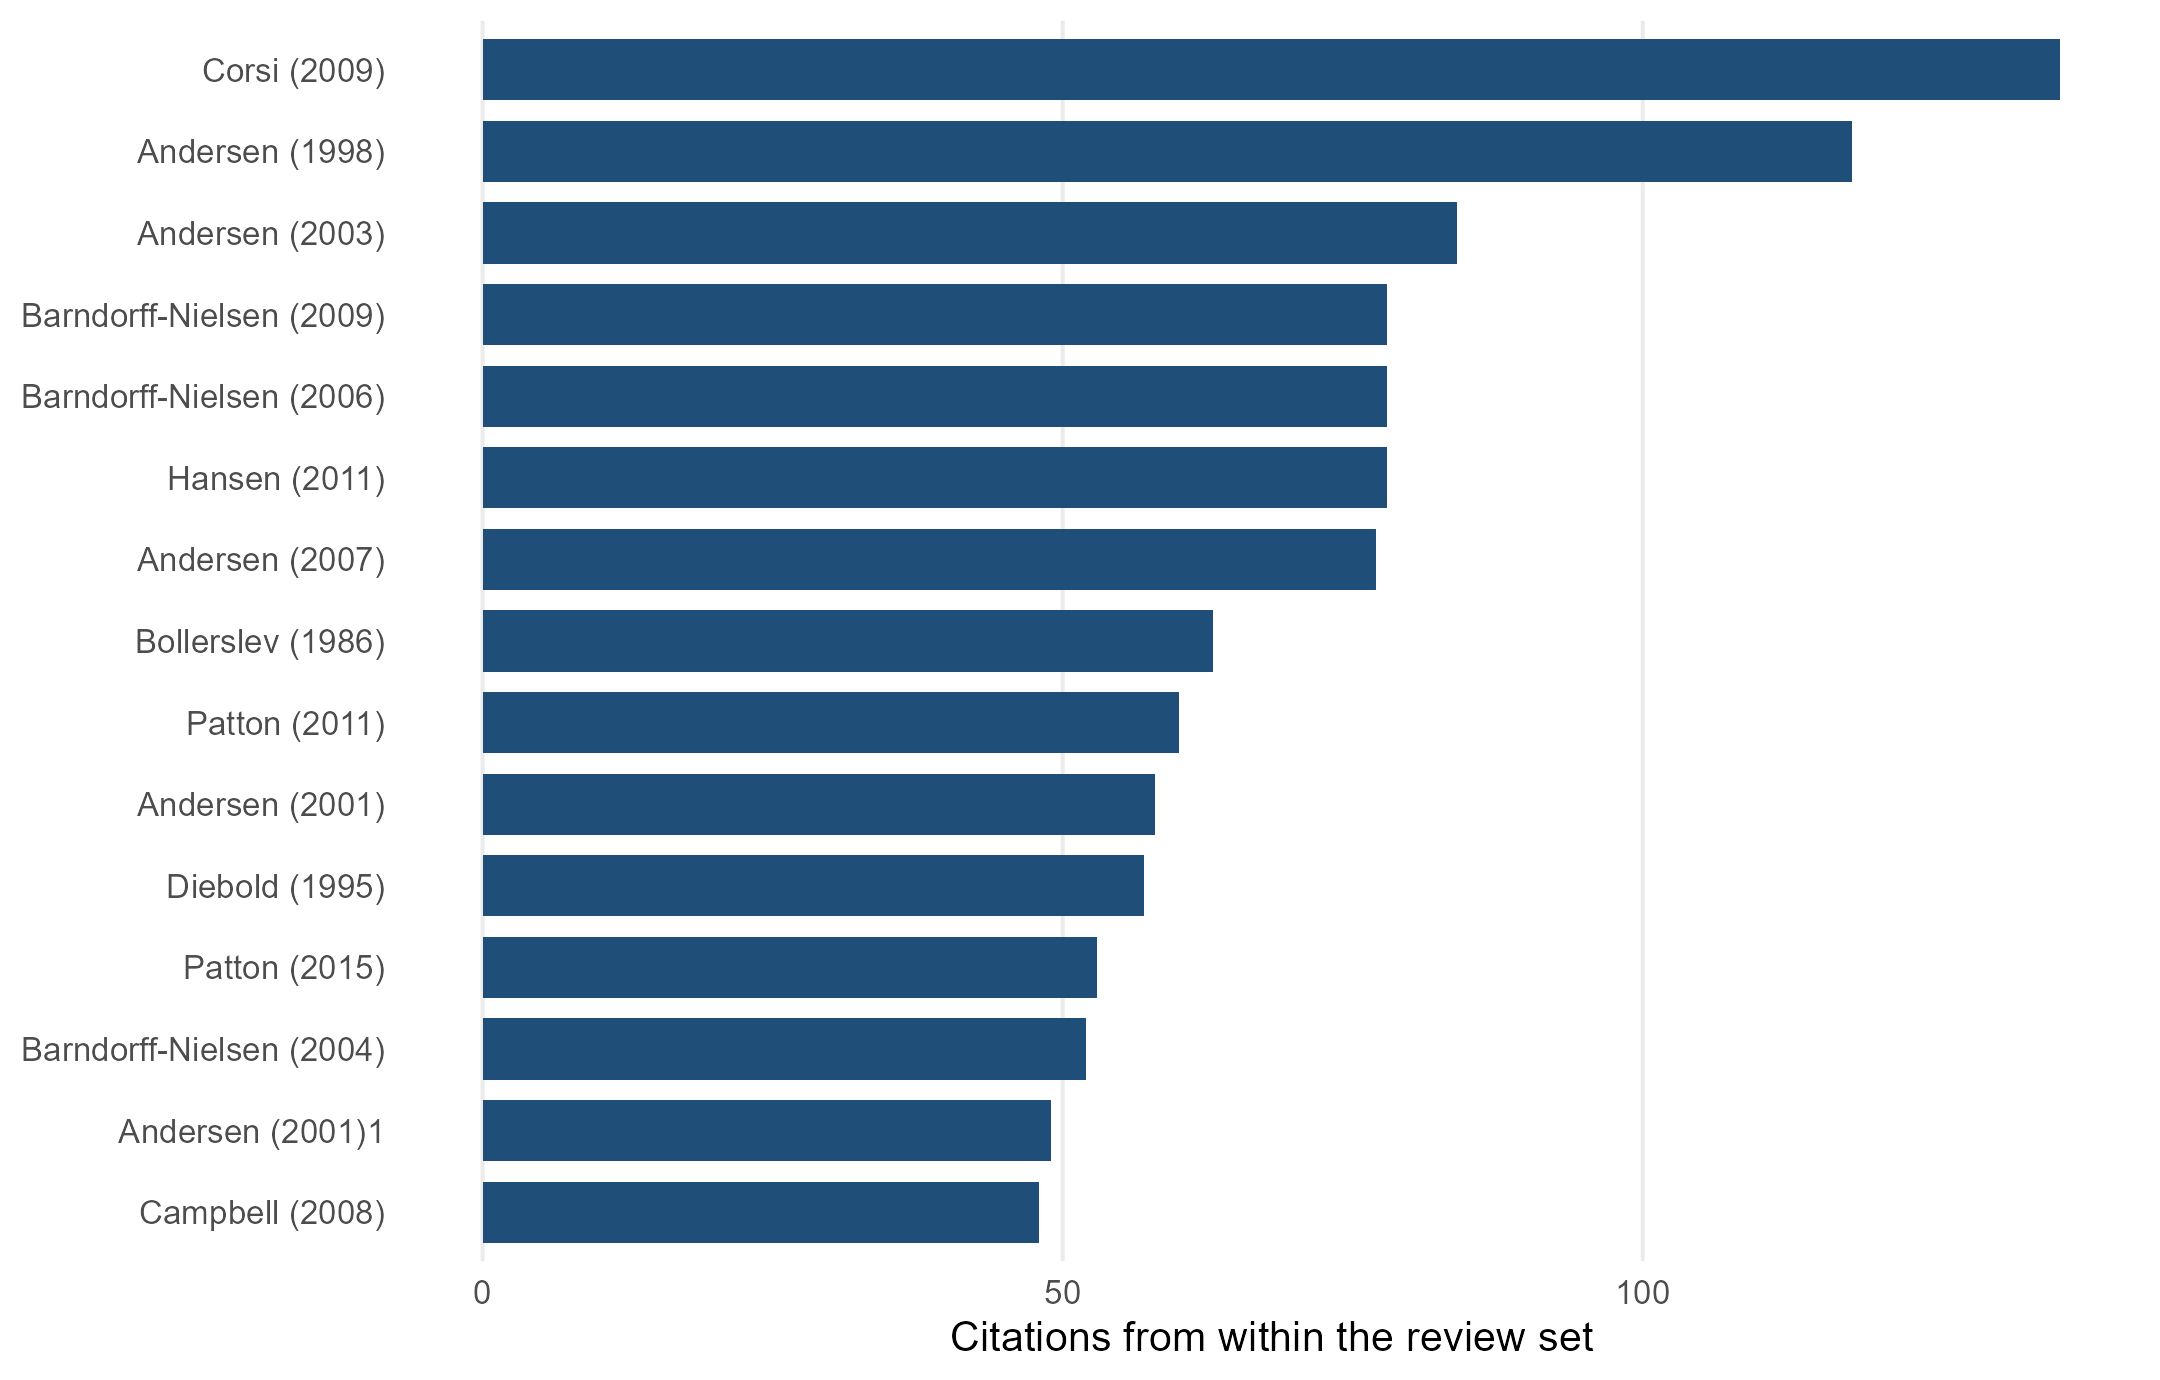
\includegraphics[width=0.86\linewidth]{figures/lit_localcited.png}
\caption{Most locally cited references}
\end{subfigure}
\begin{subfigure}{\linewidth}\centering
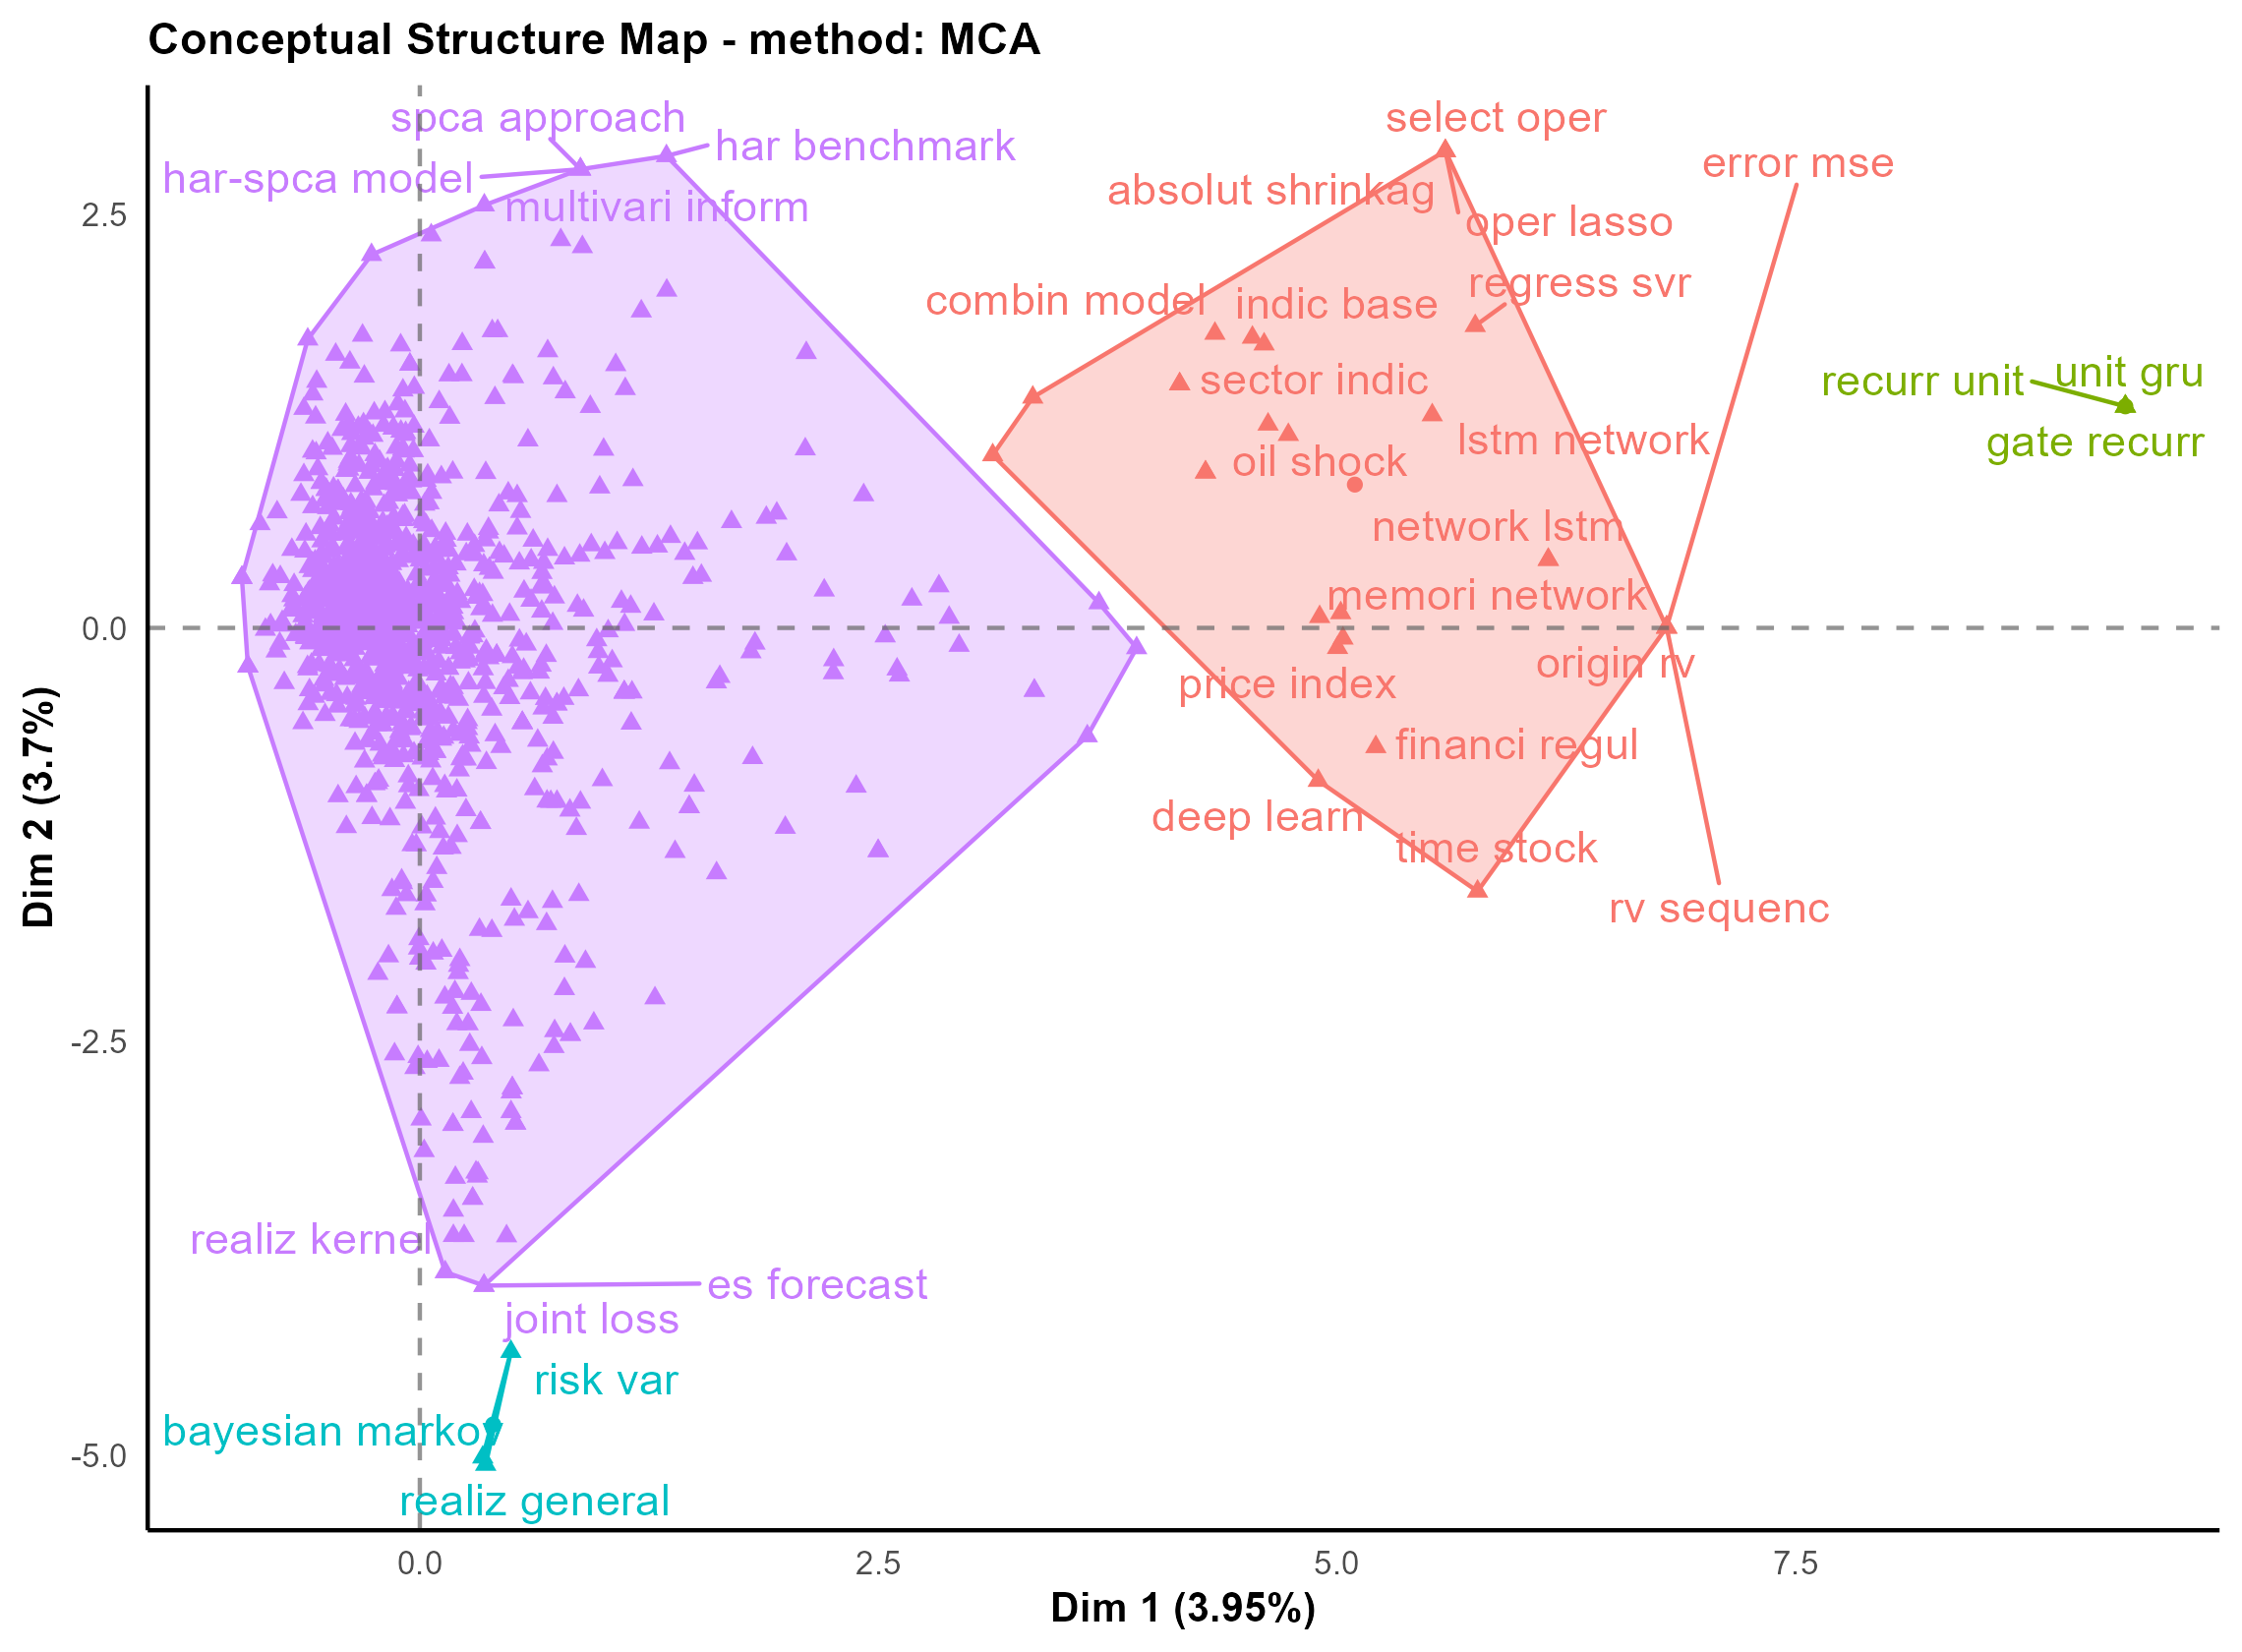
\includegraphics[width=0.72\linewidth]{figures/lit_conceptual.png}
\caption{Conceptual structure map}
\end{subfigure}
\label{fig:litstructure}
\end{figure}
